\documentclass[12pt,a4paper]{ctexart}
\usepackage{graphicx}
\usepackage{wrapfig}
\usepackage{float}
\usepackage{siunitx}
\usepackage{subfigure}
\usepackage{caption}
\usepackage{natbib}
\usepackage{listings} % 引入listings宏包用于插入代码
\usepackage{xcolor} % 引入xcolor宏包以支持更多的颜色设置

% 设置Verilog代码样式
\lstdefinestyle{verilog}{
    language=Verilog, % 设置语言为Verilog
    basicstyle=\small\ttfamily, % 设置基本字体样式
    keywordstyle=\color{blue}, % 关键字颜色设置
    commentstyle=\color{gray}\ttfamily, % 注释颜色和样式设置
    stringstyle=\color{red!60!black},
    numbers=left, % 行号在左边显示
    numberstyle=\tiny,
    frame=single, % 添加单线框
    rulecolor=\color{black!30}, % 边框颜色
    breaklines=true, % 允许自动换行
}

\title{实验 5:无冒险流水线 CPU}
\author{张子康 \ PB22020660}
\date{\today}

\begin{document}
\maketitle
\newpage
\section{实验目的与内容}
\subsection{实验目的}
将上一次实验设计的 CPU 流水化,形成一个不考虑冒险的流水线 CPU。
\subsection{实验内容}
\subsubsection{任务 1:写优先的寄存器堆}
根据实验文档中的介绍将寄存器堆改为写优先的模式,并仿真测试正确性。
\subsubsection{任务 2:无冒险流水线}
正确设计并例化四个段间寄存器,连线以实现无冒险流水线 CPU。最终,你需要在 FPGAOL 上上板运行,并通过我们给出的测试程序。
\section{逻辑设计}
\begin{figure}[H]
    \centering
    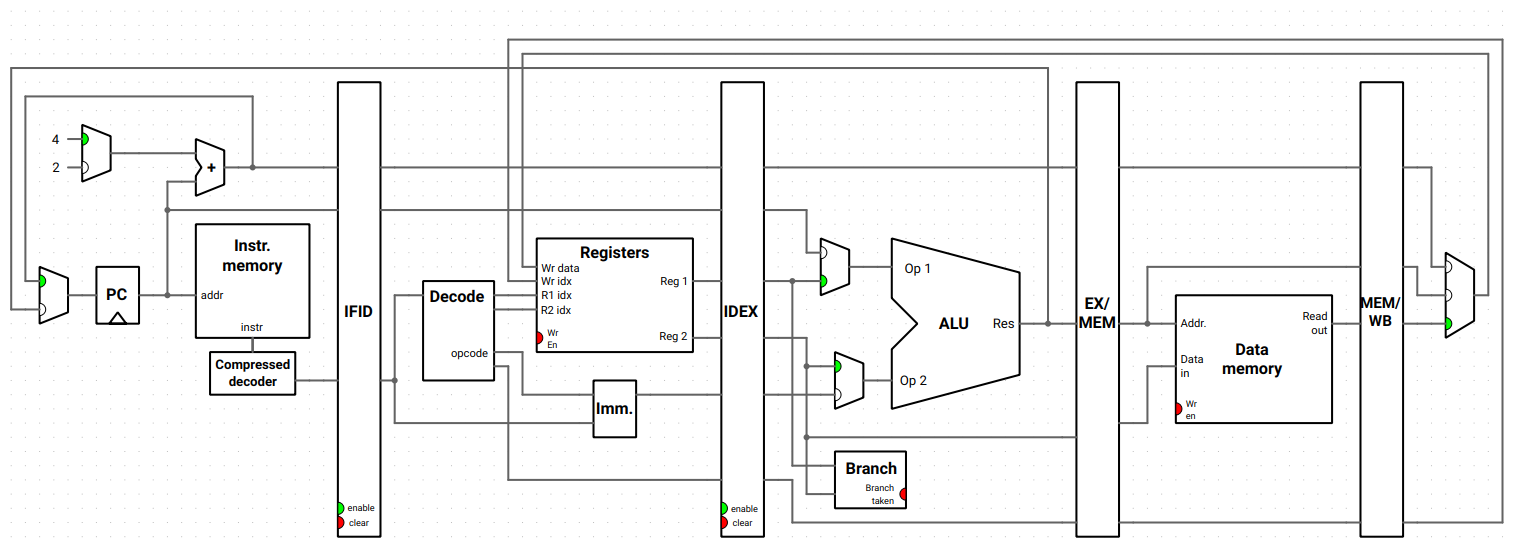
\includegraphics[scale=0.4]{pic/数据通路.png}
    \caption{无冒险五级流水线数据通路}
\end{figure}
\subsection{任务 1:写优先的寄存器堆}
写优先寄存器堆的实现如下:
\begin{lstlisting}[style=verilog]
module REG_FILE (input [0 : 0] clk,
                 input [4 : 0] rf_ra0,
                 input [4 : 0] rf_ra1,
                 input [4 : 0] rf_wa,
                 input [0 : 0] rf_we,
                 input [31 : 0] rf_wd,
                 output [31 : 0] rf_rd0,
                 output [31 : 0] rf_rd1,
                 input [4:0] debug_reg_ra,
                 output [31:0] debug_reg_rd);

reg [31 : 0] reg_file [0 : 31];

// 用于初始化寄存器
integer i;
initial begin
    for (i = 0; i < 32; i = i + 1)
        reg_file[i] = 0;
end

// 写优先
assign rf_rd0 = (rf_ra0==rf_wa && rf_ra0!=5'b00000 && rf_we)?rf_wd : reg_file[rf_ra0];
assign rf_rd1 = (rf_ra1==rf_wa && rf_ra1!=5'b00000 && rf_we)?rf_wd : reg_file[rf_ra1];

assign debug_reg_rd = /*(debug_reg_ra==rf_wa && debug_reg_ra!=5'b00000 && rf_we)?rf_wd : */reg_file[debug_reg_ra];

always @(posedge clk) begin
    if (rf_we && rf_wa != 5'd00000)
        reg_file[rf_wa] <= rf_wd;
    else
        reg_file[rf_wa] <= reg_file[rf_wa];
end

endmodule
\end{lstlisting}
若没有使用写优先寄存器堆,给定程序结果如下:
x4=32'H0000000c,x5=32'H00000017。
\subsection{任务 2:无冒险流水线}
段间寄存器实现如下(以IF\underline{~}ID为例,其他段间寄存器实现相同,仅模块命名有区别):
\begin{lstlisting}[style=verilog]
// 含_in后缀的为输入信号,含_out后缀的为输出信号
// 信号一旦产生就向后传输
module ID_EX(
    input clk,
    input rst,
    input flush,
    input stall,
    input en,
    // PC
    input [31:0] pc_add4_in,
    input [31:0] pc_in,

    output [31:0] pc_add4_out,
    output [31:0] pc_out,

    // INST
    input [31:0] inst_in,

    output [31:0] inst_out,
    
    // DECODER
    input [4:0] alu_op_in,
    input [3:0] dmem_access_in,
    input [31:0] imm_in,
    input [4:0] rf_ra0_in,
    input [4:0] rf_ra1_in,
    input [4:0] rf_wa_in,
    input [0:0] rf_we_in,
    input [1:0] rf_wd_sel_in,
    input [0:0] alu_src0_sel_in,
    input [0:0] alu_src1_sel_in,
    input [3:0] br_type_in,
    input [0:0] dmem_we_in,

    output [4:0] alu_op_out,
    output [3:0] dmem_access_out,
    output [31:0] imm_out,
    output [4:0] rf_ra0_out,
    output [4:0] rf_ra1_out,
    output [4:0] rf_wa_out,
    output [0:0] rf_we_out,
    output [1:0] rf_wd_sel_out,
    output [0:0] alu_src0_sel_out,
    output [0:0] alu_src1_sel_out,
    output [3:0] br_type_out,
    output [0:0] dmem_we_out,

    // REG_FILE
    input [31:0] rf_rd0_in,
    input [31:0] rf_rd1_in,

    output [31:0] rf_rd0_out,
    output [31:0] rf_rd1_out,

    // MUX1
    input [31:0] alu_src0_in,
    input [31:0] alu_src1_in,

    output [31:0] alu_src0_out,
    output [31:0] alu_src1_out,

    // NPC
    input [31:0] npc_in,

    output [31:0] npc_out,
    // BRANCH
    input [1 : 0] npc_sel_in,
    
    output [1 : 0] npc_sel_out,
    // ALU
    input [31:0] alu_res_in,
    
    output [31:0] alu_res_out,

    // SLU
    input [31:0] dmem_rd_out_in,
    input [31:0] dmem_wdata_mem_in,

    output [31:0] dmem_rd_out_out,
    output [31:0] dmem_wdata_mem_out,

    // DM
    input [31:0] dmem_rdata_mem_in,

    output [31:0] dmem_rdata_mem_out,

    // COMMIT
    input [0:0] commit_in,
    
    output [0:0] commit_out
);
    reg [31:0] pc_add4;
    reg [31:0] pc;
    reg [31:0] inst;

    reg [4:0] alu_op;
    reg [3:0] dmem_access;
    reg [31:0] imm;
    reg [4:0] rf_ra0;
    reg [4:0] rf_ra1;
    reg [4:0] rf_wa;
    reg [0:0] rf_we;
    reg [1:0] rf_wd_sel;
    reg [0:0] alu_src0_sel;
    reg [0:0] alu_src1_sel;
    reg [3:0] br_type;
    reg [0:0] dmem_we;
    reg [31:0] rf_rd0;
    reg [31:0] rf_rd1;
    reg [0:0] commit;

    reg [31:0] alu_src0;
    reg [31:0] alu_src1;
    reg [31:0] npc;
    reg [1:0] npc_sel;
    reg [31:0] alu_res;

    reg [31:0] dmem_rd_out;
    reg [31:0] dmem_wdata_mem;
    reg [31:0] dmem_rdata_mem;

    initial begin
        commit=0;
        pc_add4=0;
        pc=32'h00400000;
        inst=0;

        alu_op=5'b11111;
        dmem_access=0;
        imm=0;
        rf_ra0=0;
        rf_ra1=0;
        rf_wa=0;
        rf_we=0;
        rf_wd_sel=0;
        alu_src0_sel=0;
        alu_src1_sel=0;
        br_type=4'b1111;
        dmem_we=0;
        rf_rd0=0;
        rf_rd1=0;
        
        alu_src0=0;
        alu_src1=0;
        npc=0;
        npc_sel=0;
        alu_res=0;

        dmem_rd_out=0;
        dmem_wdata_mem=0;
        dmem_rdata_mem=0;
    end

    assign commit_out=commit;
    assign pc_add4_out=pc_add4;
    assign pc_out=pc;
    assign inst_out=inst;
    
    assign alu_op_out=alu_op;
    assign dmem_access_out=dmem_access;
    assign imm_out=imm;
    assign rf_ra0_out=rf_ra0;
    assign rf_ra1_out=rf_ra1;
    assign rf_wa_out=rf_wa;
    assign rf_we_out=rf_we;
    assign rf_wd_sel_out=rf_wd_sel;
    assign alu_src0_sel_out=alu_src0_sel;
    assign alu_src1_sel_out=alu_src1_sel;
    assign br_type_out=br_type;
    assign dmem_we_out=dmem_we;
    assign rf_rd0_out=rf_rd0;
    assign rf_rd1_out=rf_rd1;

    assign alu_src0_out=alu_src0;
    assign alu_src1_out=alu_src1;
    assign npc_out=npc;
    assign npc_sel_out=npc_sel;
    assign alu_res_out=alu_res;
    assign dmem_rd_out_out=dmem_rd_out;
    assign dmem_wdata_mem_out=dmem_wdata_mem;
    assign dmem_rdata_mem_out=dmem_rdata_mem;

    always @(posedge clk) begin
        // 复位信号
        if(rst)begin
            commit<=0;
            pc_add4<=0;
            pc<=32'h00400000;
            inst<=0;

            alu_op<=5'b11111;
            dmem_access<=0;
            imm<=0;
            rf_ra0<=0;
            rf_ra1<=0;
            rf_wa<=0;
            rf_we<=0;
            rf_wd_sel<=0;
            alu_src0_sel<=0;
            alu_src1_sel<=0;
            br_type<=4'b1111;
            dmem_we<=0;
            rf_rd0=0;
            rf_rd1=0;

            alu_src0<=0;
            alu_src1<=0;
            npc<=0;
            npc_sel<=0;
            alu_res<=0;

            dmem_rd_out<=0;
            dmem_wdata_mem<=0;
            dmem_rdata_mem<=0;
        end
        else if(en)begin
            // flush信号
            if(flush)begin
                commit<=0;
                pc_add4<=0;
                pc<=32'h00400000;
                inst<=0;

                alu_op<=5'b11111;
                dmem_access<=0;
                imm<=0;
                rf_ra0<=0;
                rf_ra1<=0;
                rf_wa<=0;
                rf_we<=0;
                rf_wd_sel<=0;
                alu_src0_sel<=0;
                alu_src1_sel<=0;
                br_type<=4'b1111;
                dmem_we<=0;
                rf_rd0=0;
                rf_rd1=0;

                alu_src0<=0;
                alu_src1<=0;
                npc<=0;
                npc_sel<=0;
                alu_res<=0;

                dmem_rd_out<=0;
                dmem_wdata_mem<=0;
                dmem_rdata_mem<=0;
            end
            // stall信号
            else if(stall)begin
                commit<=commit;

                pc_add4<=pc_add4;
                pc<=pc;
                inst<=inst;

                alu_op<=alu_op;
                dmem_access<=dmem_access;
                imm<=imm;
                rf_ra0<=rf_ra0;
                rf_ra1<=rf_ra1;
                rf_wa<=rf_wa;
                rf_we<=rf_we;
                rf_wd_sel<=rf_wd_sel;
                alu_src0_sel<=alu_src0_sel;
                alu_src1_sel<=alu_src1_sel;
                br_type<=br_type;
                dmem_we<=dmem_we;
                rf_rd0<=rf_rd0;
                rf_rd1<=rf_rd1;

                alu_src0<=alu_src0;
                alu_src1<=alu_src1;
                npc<=npc;
                npc_sel<=npc_sel;
                alu_res<=alu_res;

                dmem_rd_out<=dmem_rd_out;
                dmem_wdata_mem<=dmem_wdata_mem;
                dmem_rdata_mem<=dmem_rdata_mem;
            end 
            // 在写使能且不进行复位,flush,stall情况下,
            // 更新寄存器的值
            else begin
                commit<=commit_in;

                pc_add4<=pc_add4_in;
                pc<=pc_in;
                inst<=inst_in;

                alu_op<=alu_op_in;
                dmem_access<=dmem_access_in;
                imm<=imm_in;
                rf_ra0<=rf_ra0_in;
                rf_ra1<=rf_ra1_in;
                rf_wa<=rf_wa_in;
                rf_we<=rf_we_in;
                rf_wd_sel<=rf_wd_sel_in;
                alu_src0_sel<=alu_src0_sel_in;
                alu_src1_sel<=alu_src1_sel_in;
                br_type<=br_type_in;
                dmem_we<=dmem_we_in;
                rf_rd0=rf_rd0_in;
                rf_rd1=rf_rd1_in;

                alu_src0<=alu_src0_in;
                alu_src1<=alu_src1_in;
                npc<=npc_in;
                npc_sel<=npc_sel_in;
                alu_res<=alu_res_in;

                dmem_rd_out<=dmem_rd_out_in;
                dmem_wdata_mem<=dmem_wdata_mem_in;
                dmem_rdata_mem<=dmem_rdata_mem_in;
            end
        end
        else begin
            commit<=commit;

            pc_add4<=pc_add4;
            pc<=pc;
            inst<=inst;

            alu_op<=alu_op;
            dmem_access<=dmem_access;
            imm<=imm;
            rf_ra0<=rf_ra0;
            rf_ra1<=rf_ra1;
            rf_wa<=rf_wa;
            rf_we<=rf_we;
            rf_wd_sel<=rf_wd_sel;
            alu_src0_sel<=alu_src0_sel;
            alu_src1_sel<=alu_src1_sel;
            br_type<=br_type;
            dmem_we<=dmem_we;
            rf_rd0=rf_rd0;
            rf_rd1=rf_rd1;

            alu_src0<=alu_src0;
            alu_src1<=alu_src1;
            npc<=npc;
            npc_sel<=npc_sel;
            alu_res<=alu_res;

            dmem_rd_out<=dmem_rd_out;
            dmem_wdata_mem<=dmem_wdata_mem;
            dmem_rdata_mem<=dmem_rdata_mem;
        end
    end
endmodule
\end{lstlisting}
对于无用的输入,在例化时将其端口置 0。\par
CPU模块如下:
\begin{lstlisting}[style=verilog]
`include "./include/config.v"

module CPU (input [0 : 0] clk,
            input [0 : 0] rst,
            input [0 : 0] global_en,
            output [31 : 0] imem_raddr,
            input [31 : 0] imem_rdata,
            input [31 : 0] dmem_rdata,      // Unused
            output [0 : 0] dmem_we,        // Unused
            output [31 : 0] dmem_addr,      // Unused
            output [31 : 0] dmem_wdata,     // Unused
            output [0 : 0] commit,
            output [31 : 0] commit_pc,
            output [31 : 0] commit_inst,
            output [0 : 0] commit_halt,
            output [0 : 0] commit_reg_we,
            output [4 : 0] commit_reg_wa,
            output [31 : 0] commit_reg_wd,
            output [0 : 0] commit_dmem_we,
            output [31 : 0] commit_dmem_wa,
            output [31 : 0] commit_dmem_wd,
            input [4 : 0] debug_reg_ra,
            output [31 : 0] debug_reg_rd);
    
    
    // 定义所需的网线
    wire [0:0] commit_if;
    wire [31:0] pc_if;
    wire [31:0] pcadd4_if;
    wire [31:0] inst_if;
    
    wire [0:0] commit_id;
    wire [31:0] pc_id;
    wire [31:0] pcadd4_id;
    wire [31:0] inst_id;
    wire [4:0] alu_op_id;
    wire [3:0] dmem_access_id;
    wire [31:0] imm_id;
    wire [4:0] rf_ra0_id;
    wire [4:0] rf_ra1_id;
    wire [5:0] rf_wa_id;
    wire [0:0] rf_we_id;
    wire [1:0] rf_wd_sel_id;
    wire [0:0] alu_src0_sel_id;
    wire [0:0] alu_src1_sel_id;
    wire [3:0] br_type_id;
    wire [0:0] dmem_we_id;
    wire [31:0] rf_rd0_id;
    wire [31:0] rf_rd1_id;

    wire [0:0] commit_ex;
    wire [31:0] pc_ex;
    wire [31:0] pcadd4_ex;
    wire [31:0] inst_ex;
    wire [4:0] alu_op_ex;
    wire [3:0] dmem_access_ex;
    wire [31:0] imm_ex;
    wire [4:0] rf_ra0_ex;
    wire [4:0] rf_ra1_ex;
    wire [5:0] rf_wa_ex;
    wire [0:0] rf_we_ex;
    wire [1:0] rf_wd_sel_ex;
    wire [0:0] alu_src0_sel_ex;
    wire [0:0] alu_src1_sel_ex;
    wire [3:0] br_type_ex;
    wire [0:0] dmem_we_ex;
    wire [31:0] rf_rd0_ex;
    wire [31:0] rf_rd1_ex;
    wire [31:0] npc_ex;
    wire [31:0] pc_j_ex;
    wire [31:0] alu_src0_ex;
    wire [31:0] alu_src1_ex;
    wire [31:0] alu_res_ex;
    wire [1:0] npc_sel_ex;

    wire [0:0] commit_mem;
    wire [31:0] pc_mem;
    wire [31:0] pcadd4_mem;
    wire [31:0] inst_mem;
    wire [4:0] alu_op_mem;
    wire [3:0] dmem_access_mem;
    wire [31:0] imm_mem;
    wire [4:0] rf_ra0_mem;
    wire [4:0] rf_ra1_mem;
    wire [5:0] rf_wa_mem;
    wire [0:0] rf_we_mem;
    wire [1:0] rf_wd_sel_mem;
    wire [0:0] alu_src0_sel_mem;
    wire [0:0] alu_src1_sel_mem;
    wire [3:0] br_type_mem;
    wire [0:0] dmem_we_mem;
    wire [31:0] rf_rd0_mem;
    wire [31:0] rf_rd1_mem;
    wire [31:0] npc_mem;
    wire [31:0] pc_j_mem;
    wire [31:0] alu_src0_mem;
    wire [31:0] alu_src1_mem;
    wire [31:0] alu_res_mem;
    wire [31:0] dmem_rd_out_mem;
    wire [31:0] dmem_wdata_mem;
    wire [31:0] dmem_rdata_mem;
    wire [1:0] npc_sel_mem;

    wire [0:0] commit_wb;
    wire [31:0] pc_wb;
    wire [31:0] pcadd4_wb;
    wire [31:0] inst_wb;
    wire [4:0] alu_op_wb;
    wire [3:0] dmem_access_wb;
    wire [31:0] imm_wb;
    wire [4:0] rf_ra0_wb;
    wire [4:0] rf_ra1_wb;
    wire [5:0] rf_wa_wb;
    wire [0:0] rf_we_wb;
    wire [1:0] rf_wd_sel_wb;
    wire [0:0] alu_src0_sel_wb;
    wire [0:0] alu_src1_sel_wb;
    wire [3:0] br_type_wb;
    wire [0:0] dmem_we_wb;
    wire [31:0] rf_rd0_wb;
    wire [31:0] rf_rd1_wb;
    wire [31:0] npc_wb;
    wire [31:0] pc_j_wb;
    wire [31:0] alu_src0_wb;
    wire [31:0] alu_src1_wb;
    wire [31:0] alu_res_wb;
    wire [31:0] dmem_rd_out_wb;
    wire [31:0] dmem_wdata_wb;
    wire [31:0] dmem_rdata_wb;
    wire [31:0] rf_wd_wb;
    wire [1:0] npc_sel_wb;

    wire flush,stall,en;
    wire flush_if_id,flush_id_ex,flush_ex_mem,flush_mem_wb;

    assign commit_if = 1;
    assign stall = 0;
    assign en = global_en;
    // assign global_en  = !(inst_if == 32'H00100073);
    assign imem_raddr = (pc_if-32'h00400000)/'d4;
    assign inst_if   = imem_rdata;
    assign pc_j_ex       = alu_res_ex&~1;
    assign dmem_wd_in = rf_rd1_mem;
    assign dmem_we    = dmem_we_mem;
    assign dmem_addr  = (alu_res_mem-32'h10010000)/'d4;
    assign dmem_wdata = dmem_wdata_mem;
    assign dmem_rdata_mem = dmem_rdata;

    // 控制各个段间寄存器的flush信号
    assign flush_if_id=inst_if==32'h00000013 && inst_id==32'h00000013;
    assign flush_id_ex=inst_if==32'h00000013 && inst_id==32'h00000013;
    assign flush_ex_mem=0;
    assign flush_mem_wb=0;

    // 例化各个模块
    PC_PLUS4 pc_plus(
        .pc(pc_if),
        .pc_plus4(pcadd4_if)
    );
    
    PC pc(
        .clk    (clk),
        .rst    (rst),
        .en     (global_en),    // 当 global_en 为高电平时,PC 才会更新,CPU 才会执行指令。
        .npc    (npc_ex),
        .pc     (pc_if)
    );

    IF_ID if_id(
        .clk(clk),
        .rst(rst),
        .flush(flush_if_id),
        .stall(stall),
        .en(en),
        //PC
        .pc_add4_in(pcadd4_if),
        .pc_in(pc_if),
        .pc_add4_out(pcadd4_id),
        .pc_out(pc_id),
        //INST
        .inst_in(inst_if),
        .inst_out(inst_id),
        //DECODER
        .alu_op_in(0),
        .dmem_access_in(0),
        .imm_in(0),
        .rf_ra0_in(0),
        .rf_ra1_in(0),
        .rf_wa_in(0),
        .rf_we_in(0),
        .rf_wd_sel_in(0),
        .alu_src0_sel_in(0),
        .alu_src1_sel_in(0),
        .br_type_in(0),
        .dmem_we_in(0),
        .alu_op_out(),
        .dmem_access_out(),
        .imm_out(),
        .rf_ra0_out(),
        .rf_ra1_out(),
        .rf_wa_out(),
        .rf_we_out(),
        .rf_wd_sel_out(),
        .alu_src0_sel_out(),
        .alu_src1_sel_out(),
        .br_type_out(),
        .dmem_we_out(),
        //REG_FILE
        .rf_rd0_in(0),
        .rf_rd1_in(0),
        .rf_rd0_out(),
        .rf_rd1_out(),
        //MUX1
        .alu_src0_in(0),
        .alu_src1_in(0),
        .alu_src0_out(),
        .alu_src1_out(),
        //NPC
        .npc_in(0),
        .npc_out(),
        //BRANCH
        .npc_sel_in(0),
        .npc_sel_out(),
        //ALU
        .alu_res_in(0),
        .alu_res_out(),
        //SLU
        .dmem_rd_out_in(0),
        .dmem_wdata_mem_in(0),
        .dmem_rd_out_out(),
        .dmem_wdata_mem_out(),
        //DM
        .dmem_rdata_mem_in(0),
        .dmem_rdata_mem_out(),
        .commit_in(commit_if),
        .commit_out(commit_id)
    );

    DECODER decoder(
        .inst(inst_id),
        .alu_op(alu_op_id),
        .imm(imm_id),
        .rf_ra0(rf_ra0_id),
        .rf_ra1(rf_ra1_id),
        .rf_wa(rf_wa_id),
        .rf_we(rf_we_id),
        .alu_src0_sel(alu_src0_sel_id),
        .alu_src1_sel(alu_src1_sel_id),
        .dmem_access(dmem_access_id),
        .rf_wd_sel(rf_wd_sel_id),
        .br_type(br_type_id),
        .dmem_we(dmem_we_id)
    );
    
    REG_FILE reg_file(
        .clk(clk),
        .rf_ra0(rf_ra0_id),
        .rf_ra1(rf_ra1_id),
        .rf_wa(rf_wa_wb),
        .rf_we(rf_we_wb),
        .rf_wd(rf_wd_wb),
        .rf_rd0(rf_rd0_id),
        .rf_rd1(rf_rd1_id),
        .debug_reg_rd(debug_reg_rd),
        .debug_reg_ra(debug_reg_ra)
    );
    
    ID_EX id_ex(
        .clk(clk),
        .rst(rst),
        .flush(flush_id_ex),
        .stall(stall),
        .en(en),
        //PC
        .pc_add4_in(pcadd4_id),
        .pc_in(pc_id),
        .pc_add4_out(pcadd4_ex),
        .pc_out(pc_ex),
        //INST
        .inst_in(inst_id),
        .inst_out(inst_ex),
        //DECODER
        .alu_op_in(alu_op_id),
        .dmem_access_in(dmem_access_id),
        .imm_in(imm_id),
        .rf_ra0_in(rf_ra0_id),
        .rf_ra1_in(rf_ra1_id),
        .rf_wa_in(rf_wa_id),
        .rf_we_in(rf_we_id),
        .rf_wd_sel_in(rf_wd_sel_id),
        .alu_src0_sel_in(alu_src0_sel_id),
        .alu_src1_sel_in(alu_src1_sel_id),
        .br_type_in(br_type_id),
        .dmem_we_in(dmem_we_id),
        .alu_op_out(alu_op_ex),
        .dmem_access_out(dmem_access_ex),
        .imm_out(imm_ex),
        .rf_ra0_out(rf_ra0_ex),
        .rf_ra1_out(rf_ra1_ex),
        .rf_wa_out(rf_wa_ex),
        .rf_we_out(rf_we_ex),
        .rf_wd_sel_out(rf_wd_sel_ex),
        .alu_src0_sel_out(alu_src0_sel_ex),
        .alu_src1_sel_out(alu_src1_sel_ex),
        .br_type_out(br_type_ex),
        .dmem_we_out(dmem_we_ex),
        //REG_FILE
        .rf_rd0_in(rf_rd0_id),
        .rf_rd1_in(rf_rd1_id),
        .rf_rd0_out(rf_rd0_ex),
        .rf_rd1_out(rf_rd1_ex),
        //MUX1
        .alu_src0_in(0),
        .alu_src1_in(0),
        .alu_src0_out(),
        .alu_src1_out(),
        //NPC
        .npc_in(0),
        .npc_out(),
        //BRANCH
        .npc_sel_in(0),
        .npc_sel_out(),
        //ALU
        .alu_res_in(0),
        .alu_res_out(),
        //SLU
        .dmem_rd_out_in(0),
        .dmem_wdata_mem_in(0),
        .dmem_rd_out_out(),
        .dmem_wdata_mem_out(),
        //DM
        .dmem_rdata_mem_in(0),
        .dmem_rdata_mem_out(),
        .commit_in(commit_id),
        .commit_out(commit_ex)
    );

    MUX1 mux1(
        .src0(rf_rd0_ex),
        .src1(pc_ex),
        .sel(alu_src0_sel_ex),
        .res(alu_src0_ex)
    );

    MUX1 mux2(
        .src0(rf_rd1_ex),
        .src1(imm_ex),
        .sel(alu_src1_sel_ex),
        .res(alu_src1_ex)
    );
    
    ALU alu(
        .alu_src0(alu_src0_ex),
        .alu_src1(alu_src1_ex),
        .alu_op(alu_op_ex),
        .alu_res(alu_res_ex)
    );
    
    BRANCH branch(
        .br_type(br_type_ex),
        .br_src0(rf_rd0_ex),
        .br_src1(rf_rd1_ex),
        .npc_sel(npc_sel_ex)
    );
    NPC npc(
        .pc_offset(alu_res_ex),
        .pc_add4(pcadd4_if),
        .pc_j(pc_j_ex),
        .npc_sel(npc_sel_ex),
        .npc(npc_ex)
    );

    EX_MEM ex_mem(
        .clk(clk),
        .rst(rst),
        .flush(flush_ex_mem),
        .stall(stall),
        .en(en),
        //PC
        .pc_add4_in(pcadd4_ex),
        .pc_in(pc_ex),
        .pc_add4_out(pcadd4_mem),
        .pc_out(pc_mem),
        //INST
        .inst_in(inst_ex),
        .inst_out(inst_mem),
        //DECODER
        .alu_op_in(alu_op_ex),
        .dmem_access_in(dmem_access_ex),
        .imm_in(imm_ex),
        .rf_ra0_in(rf_ra0_ex),
        .rf_ra1_in(rf_ra1_ex),
        .rf_wa_in(rf_wa_ex),
        .rf_we_in(rf_we_ex),
        .rf_wd_sel_in(rf_wd_sel_ex),
        .alu_src0_sel_in(alu_src0_sel_ex),
        .alu_src1_sel_in(alu_src1_sel_ex),
        .br_type_in(br_type_ex),
        .dmem_we_in(dmem_we_ex),
        .alu_op_out(alu_op_mem),
        .dmem_access_out(dmem_access_mem),
        .imm_out(imm_mem),
        .rf_ra0_out(rf_ra0_mem),
        .rf_ra1_out(rf_ra1_mem),
        .rf_wa_out(rf_wa_mem),
        .rf_we_out(rf_we_mem),
        .rf_wd_sel_out(rf_wd_sel_mem),
        .alu_src0_sel_out(alu_src0_sel_mem),
        .alu_src1_sel_out(alu_src1_sel_mem),
        .br_type_out(br_type_mem),
        .dmem_we_out(dmem_we_mem),
        //REG_FILE
        .rf_rd0_in(rf_rd0_ex),
        .rf_rd1_in(rf_rd1_ex),
        .rf_rd0_out(rf_rd0_mem),
        .rf_rd1_out(rf_rd1_mem),
        //MUX1
        .alu_src0_in(alu_src0_ex),
        .alu_src1_in(alu_src1_ex),
        .alu_src0_out(alu_src0_mem),
        .alu_src1_out(alu_src1_mem),
        //NPC
        .npc_in(npc_ex),
        .npc_out(npc_mem),
        //BRANCH
        .npc_sel_in(npc_sel_ex),
        .npc_sel_out(npc_sel_mem),
        //ALU
        .alu_res_in(alu_res_ex),
        .alu_res_out(alu_res_mem),
        //SLU
        .dmem_rd_out_in(0),
        .dmem_wdata_mem_in(0),
        .dmem_rd_out_out(),
        .dmem_wdata_mem_out(),
        //DM
        .dmem_rdata_mem_in(0),
        .dmem_rdata_mem_out(),
        .commit_in(commit_ex),
        .commit_out(commit_mem)
    );

    SLU slu(
        .addr(alu_res_mem),
        .dmem_access(dmem_access_mem),
        .rd_in(dmem_rdata_mem),
        .wd_in(rf_rd1_mem),
        .rd_out(dmem_rd_out_mem),
        .wd_out(dmem_wdata_mem)
    );
    
    MEM_WB mem_wb(
        .clk(clk),
        .rst(rst),
        .flush(flush_mem_wb),
        .stall(stall),
        .en(en),
        //PC
        .pc_add4_in(pcadd4_mem),
        .pc_in(pc_mem),
        .pc_add4_out(pcadd4_wb),
        .pc_out(pc_wb),
        //INST
        .inst_in(inst_mem),
        .inst_out(inst_wb),
        //DECODER
        .alu_op_in(alu_op_mem),
        .dmem_access_in(dmem_access_mem),
        .imm_in(imm_mem),
        .rf_ra0_in(rf_ra0_mem),
        .rf_ra1_in(rf_ra1_mem),
        .rf_wa_in(rf_wa_mem),
        .rf_we_in(rf_we_mem),
        .rf_wd_sel_in(rf_wd_sel_mem),
        .alu_src0_sel_in(alu_src0_sel_mem),
        .alu_src1_sel_in(alu_src1_sel_mem),
        .br_type_in(br_type_mem),
        .dmem_we_in(dmem_we_mem),
        .alu_op_out(alu_op_wb),
        .dmem_access_out(dmem_access_wb),
        .imm_out(imm_wb),
        .rf_ra0_out(rf_ra0_wb),
        .rf_ra1_out(rf_ra1_wb),
        .rf_wa_out(rf_wa_wb),
        .rf_we_out(rf_we_wb),
        .rf_wd_sel_out(rf_wd_sel_wb),
        .alu_src0_sel_out(alu_src0_sel_wb),
        .alu_src1_sel_out(alu_src1_sel_wb),
        .br_type_out(br_type_wb), 
        .dmem_we_out(dmem_we_wb),
        //REG_FILE
        .rf_rd0_in(rf_rd0_mem),
        .rf_rd1_in(rf_rd1_mem),
        .rf_rd0_out(rf_rd0_wb),
        .rf_rd1_out(rf_rd1_wb),
        //MUX1
        .alu_src0_in(alu_src0_mem),
        .alu_src1_in(alu_src1_mem),
        .alu_src0_out(alu_src0_wb),
        .alu_src1_out(alu_src1_wb),
        //NPC
        .npc_in(npc_mem),
        .npc_out(npc_wb),
        //BRANCH
        .npc_sel_in(npc_sel_mem),
        .npc_sel_out(npc_sel_wb),
        //ALU
        .alu_res_in(alu_res_mem),
        .alu_res_out(alu_res_wb),
        //SLU
        .dmem_rd_out_in(dmem_rd_out_mem),
        .dmem_wdata_mem_in(dmem_wdata_mem),
        .dmem_rd_out_out(dmem_rd_out_wb),
        .dmem_wdata_mem_out(dmem_wdata_wb),
        //DM
        .dmem_rdata_mem_in(dmem_rdata_mem),
        .dmem_rdata_mem_out(dmem_rdata_wb),
        .commit_in(commit_mem),
        .commit_out(commit_wb)
    );

    MUX2 RF_MUX(
        .src0(pcadd4_wb),
        .src1(alu_res_wb),
        .src2(dmem_rd_out_wb),
        .src3(0),
        .sel(rf_wd_sel_wb),
        .res(rf_wd_wb)
    );
    
    /* --------------------------- */
    /*           Commit            */
    /* --------------------------- */
    
    // wire [0 : 0] commit_if     ;
    // assign commit_if = 1'H1;
    
    reg  [0 : 0]   commit_reg          ;
    reg  [31 : 0]   commit_pc_reg       ;
    reg  [31 : 0]   commit_inst_reg     ;
    reg  [0 : 0]   commit_halt_reg     ;
    reg  [0 : 0]   commit_reg_we_reg   ;
    reg  [4 : 0]   commit_reg_wa_reg   ;
    reg  [31 : 0]   commit_reg_wd_reg   ;
    reg  [0 : 0]   commit_dmem_we_reg  ;
    reg  [31 : 0]   commit_dmem_wa_reg  ;
    reg  [31 : 0]   commit_dmem_wd_reg  ;
    
    always @(posedge clk) begin
        if (rst) begin
            commit_reg         <= 1'H0;
            commit_pc_reg      <= 32'H0;
            commit_inst_reg    <= 32'H0;
            commit_halt_reg    <= 1'H0;
            commit_reg_we_reg  <= 1'H0;
            commit_reg_wa_reg  <= 5'H0;
            commit_reg_wd_reg  <= 32'H0;
            commit_dmem_we_reg <= 1'H0;
            commit_dmem_wa_reg <= 32'H0;
            commit_dmem_wd_reg <= 32'H0;
        end
        else if (global_en) begin
            commit_reg          <= commit_wb;
            commit_pc_reg       <= pc_wb;
            commit_inst_reg     <= inst_wb;
            commit_halt_reg     <= inst_wb == `HALT_INST;
            commit_reg_we_reg   <= rf_we_wb;
            commit_reg_wa_reg   <= rf_wa_wb;
            commit_reg_wd_reg   <= rf_wd_wb;
            commit_dmem_we_reg  <= dmem_we_wb;
            commit_dmem_wa_reg  <= alu_res_wb;
            commit_dmem_wd_reg  <= dmem_wdata_wb;
        end
            end
            
            assign commit         = commit_reg;
            assign commit_pc      = commit_pc_reg;
            assign commit_inst    = commit_inst_reg;
            assign commit_halt    = commit_halt_reg;
            assign commit_reg_we  = commit_reg_we_reg;
            assign commit_reg_wa  = commit_reg_wa_reg;
            assign commit_reg_wd  = commit_reg_wd_reg;
            assign commit_dmem_we = commit_dmem_we_reg;
            assign commit_dmem_wa = commit_dmem_wa_reg;
            assign commit_dmem_wd = commit_dmem_wd_reg;
endmodule
\end{lstlisting}
\section{仿真结果与分析}
Testbench如下:
\begin{lstlisting}[style=verilog]
`timescale 1ns / 1ps
module TB();
reg clk;
reg rst;
wire [31:0] imem_raddr;
wire dmem_we;
wire [31 : 0]            dmem_addr;
wire [31:0] imem_rdata;
wire [31 : 0]            dmem_wdata;
wire [ 0 : 0]            commit;
wire [31 : 0]            commit_pc;
wire [31 : 0]            commit_inst;
wire [ 0 : 0]            commit_halt;
wire [ 0 : 0]            commit_reg_we;
wire [ 4 : 0]            commit_reg_wa;
wire [31 : 0]            commit_reg_wd;
wire [ 0 : 0]            commit_dmem_we;
wire [31 : 0]            commit_dmem_wa;
wire [31 : 0]            commit_dmem_wd;
wire [31 : 0]            debug_reg_rd;
wire [31:0] dmem_rdata;
CPU cpu(
    .rst (rst),
    .clk (clk),
    .global_en(1'b1),
    .debug_reg_ra(0),
    .imem_raddr(imem_raddr),
    .imem_rdata(imem_rdata),
    .dmem_we(dmem_we),
    .dmem_addr(dmem_addr),
    .dmem_wdata(dmem_wdata),
    .commit(commit),
    .commit_pc(commit_pc),
    .commit_inst(commit_inst),
    .commit_halt(commit_halt),
    .commit_reg_we(commit_reg_we),
    .commit_reg_wa(commit_reg_wa),
    .commit_reg_wd(commit_reg_wd),
    .commit_dmem_we(commit_dmem_we),
    .commit_dmem_wa(commit_dmem_wa),
    .commit_dmem_wd(commit_dmem_wd),
    .debug_reg_rd(debug_reg_rd),
    .dmem_rdata(dmem_rdata)
);

INST_MEM inst_mem (
  .a(imem_raddr),      // input wire [8 : 0] a
  .d(d),      // input wire [31 : 0] d
  .clk(clk),  // input wire clk
  .we(0),    // input wire we
  .spo(imem_rdata)  // output wire [31 : 0] spo
);
DATA_MEM data_mem (
  .a(dmem_addr),      // input wire [8 : 0] a
  .d(dmem_wdata),      // input wire [31 : 0] d
  .clk(clk),  // input wire clk
  .we(dmem_we),    // input wire we
  .spo(dmem_rdata)  // output wire [31 : 0] spo
);
localparam CLK_PERIOD = 10;
always #(CLK_PERIOD/2) clk=~clk;

initial begin
    clk=0;
    rst=0;
    #10000
    $finish;
end

endmodule
\end{lstlisting}
\begin{figure}[H]
    \centering
    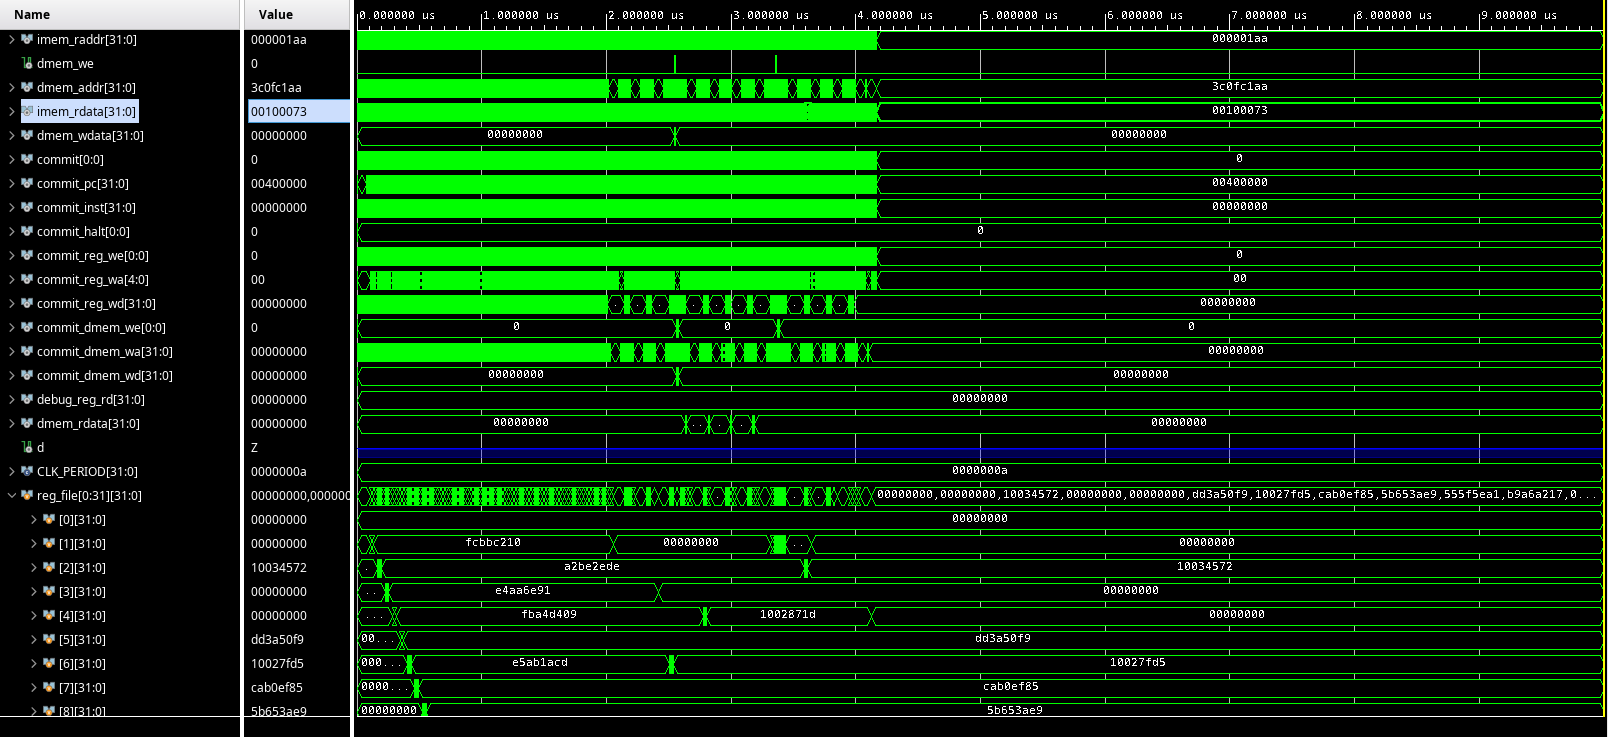
\includegraphics[scale=0.4]{pic/test1_1.png}
    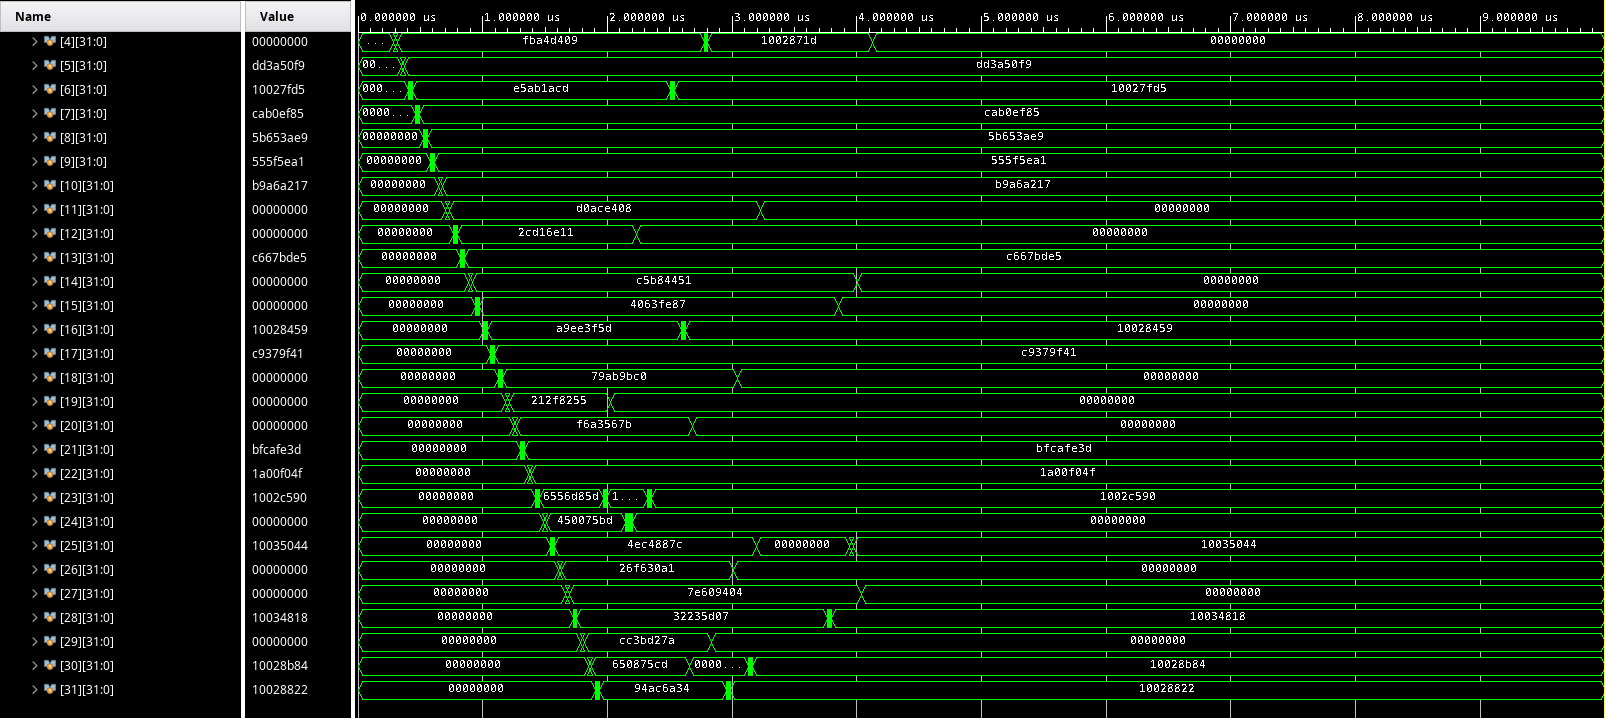
\includegraphics[scale=0.4]{pic/test1_2.png}
    \caption{测试程序 1的测试结果}
\end{figure}
\begin{figure}[H]
    \centering
    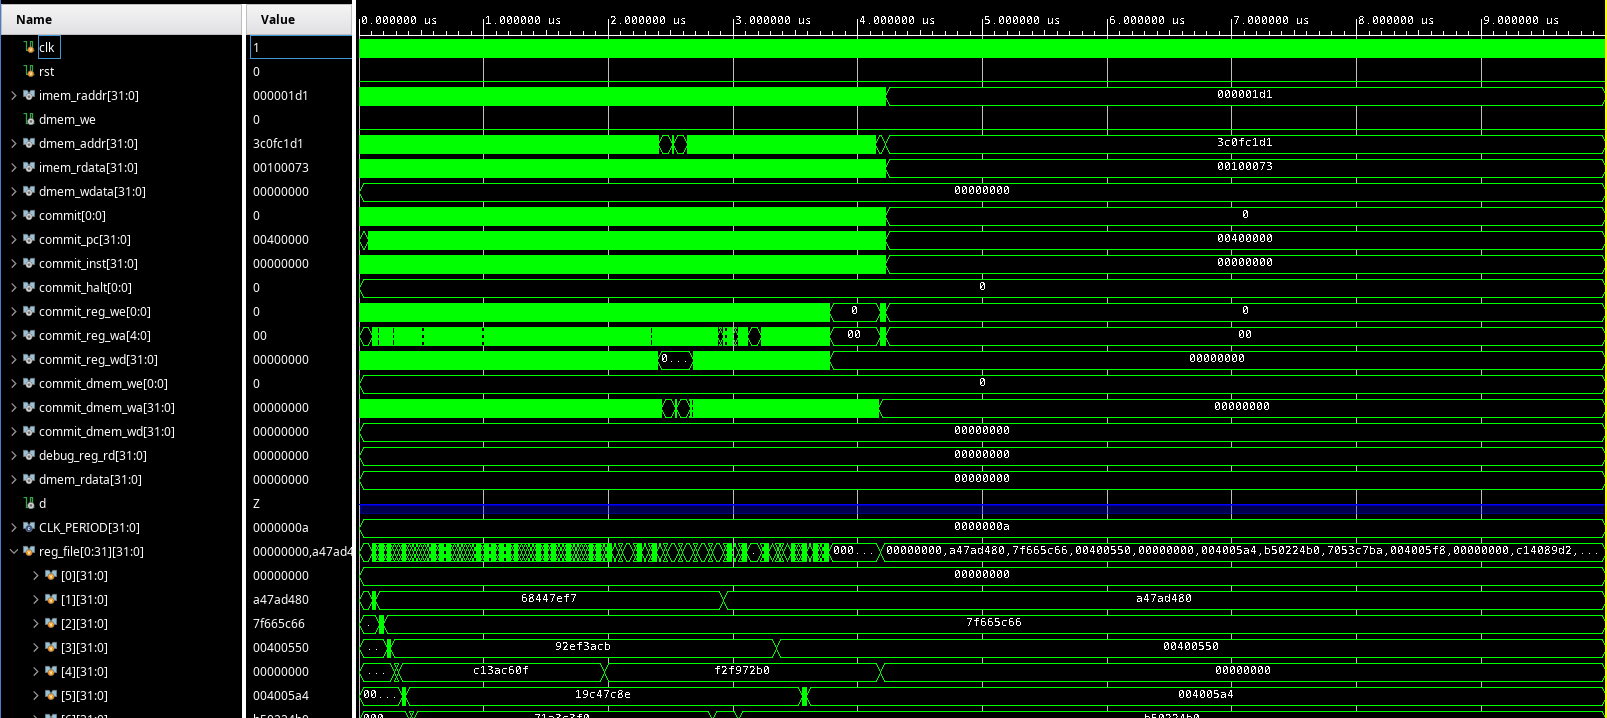
\includegraphics[scale=0.4]{pic/test2_1.png}
    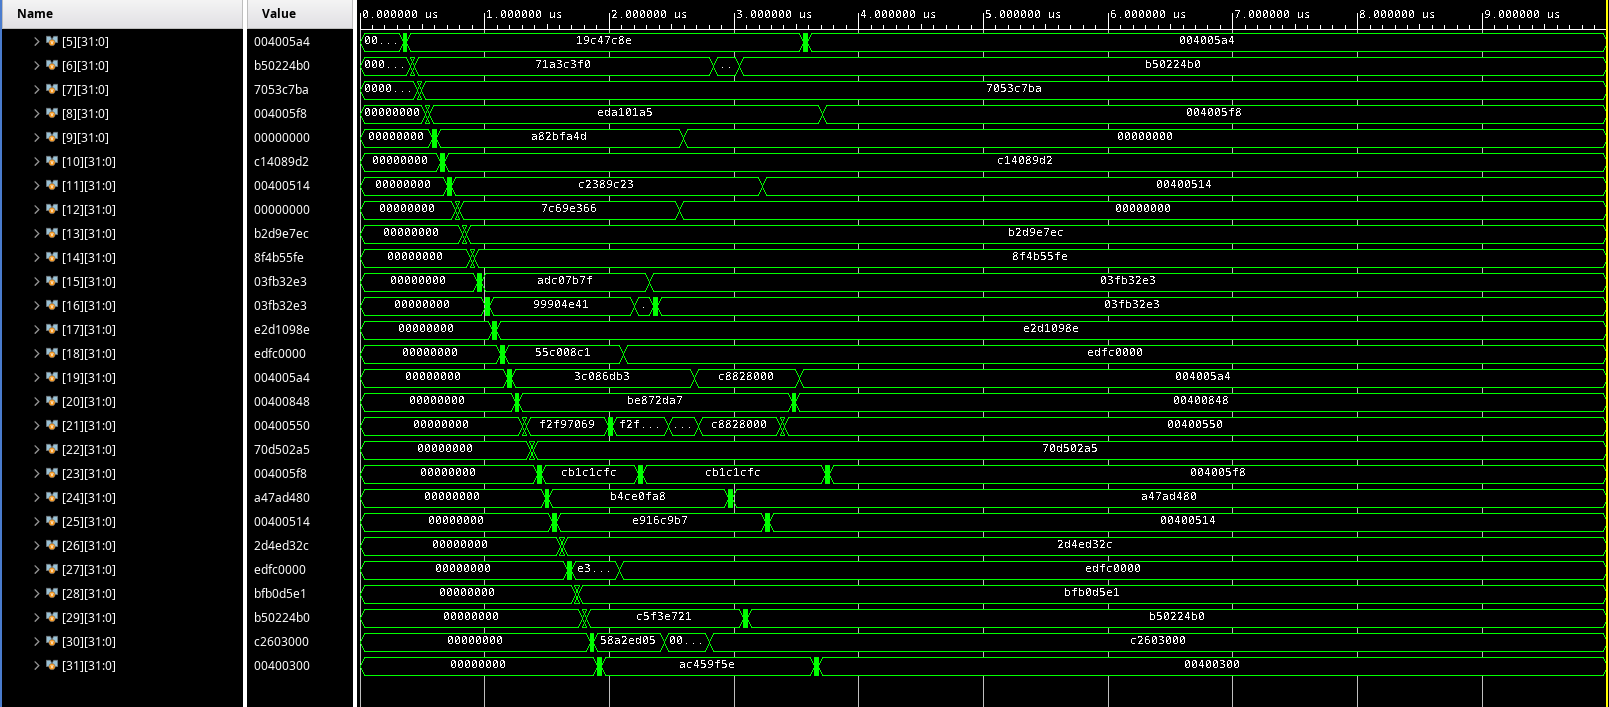
\includegraphics[scale=0.4]{pic/test2_2.png}
    \caption{测试程序 2的测试结果}
\end{figure}
仿真结果与正确结果相吻合。
\section{电路设计与分析}
\begin{figure}[H]
    \centering
    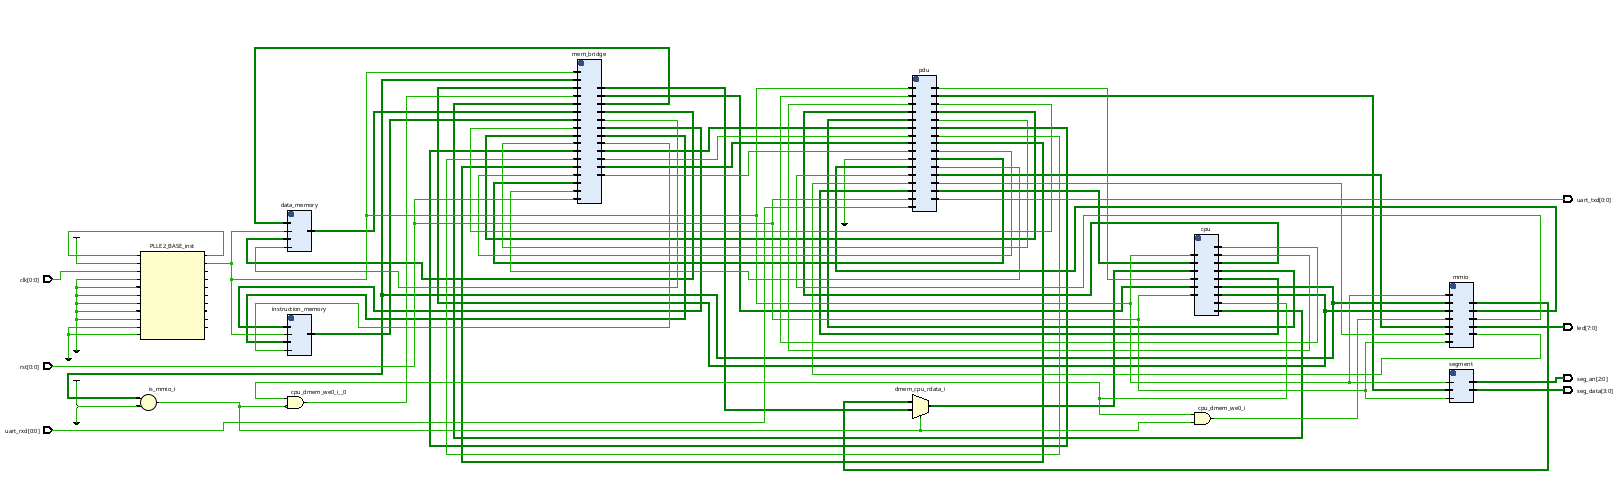
\includegraphics[scale=0.4]{pic/整体.png}
    \caption{整体的电路}
\end{figure}
\begin{figure}[H]
    \centering
    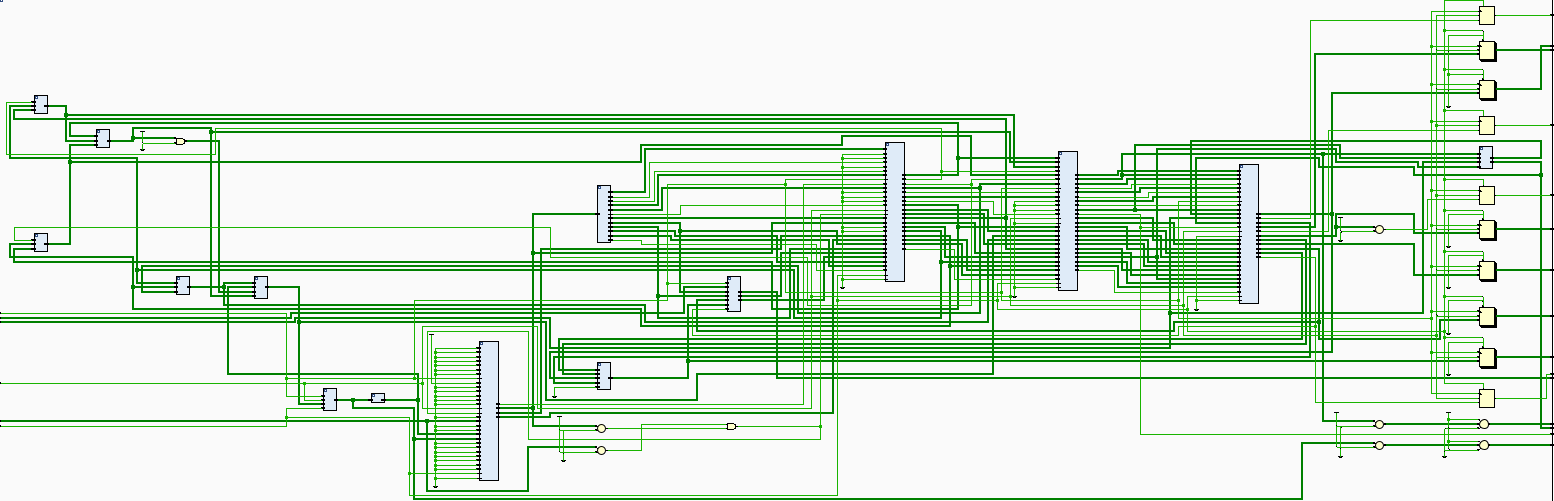
\includegraphics[scale=0.4]{pic/cpu.png}
    \caption{cpu的电路}
\end{figure}
\section{测试结果与分析}
\begin{figure}[H]
    \centering
    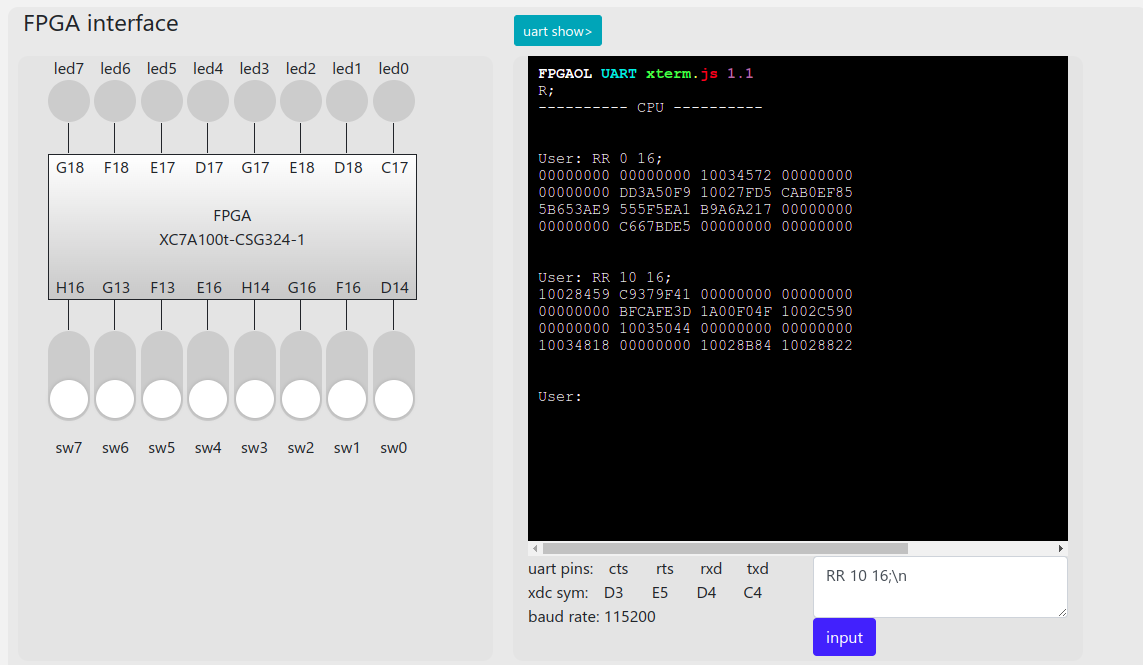
\includegraphics[scale=0.5]{pic/上板1.png}
    \caption{测试程序1上板结果}
\end{figure}
\begin{figure}[H]
    \centering
    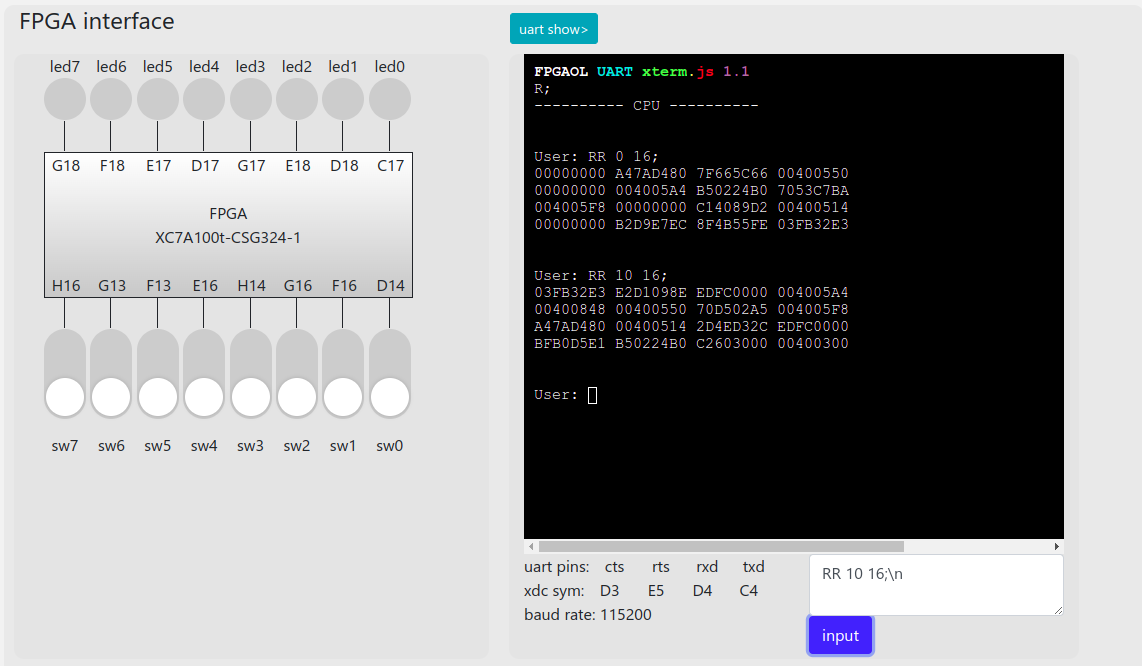
\includegraphics[scale=0.5]{pic/上板2.png}
    \caption{测试程序2上板结果}
\end{figure}
上板结果与正确结果相吻合。
\section{总结}
本次实验设计了一个不考虑冒险的流水线CPU,实现了写优先的寄存器堆和段间寄存器。
\end{document}